\documentclass{article}
\usepackage{ctex}
\usepackage{listings}
\usepackage{color}
\usepackage{xcolor}
\usepackage{hyperref}
\usepackage{graphicx}
\usepackage[a4paper, margin=1.5cm]{geometry}
% 设置 listings 参数
\lstset{
    language=C++,
    basicstyle=\ttfamily\small,
    keywordstyle=\color{blue},
    commentstyle=\color{gray},
    stringstyle=\color{red},
    breaklines=true,
    numbers=left,
    numberstyle=\tiny,
    frame=single,
    tabsize=4,
    showspaces=false,
}

\begin{document}
\title{Report for Final-term Lab: Hashmap}
\author{高南新\ 刘欣逸\ 邓皓云}
\date{May 19th, 2025}
\maketitle

\section{实验背景}
HashMap是一种非常实用的数据结构,它通过哈希函数将键映射到存储位置,从而实现快速查找。在实际开发中,
HashMap被广泛应用于各种场景,如缓存、数据库索引、符号表等。掌握HashMap的实现原理和使用方法,对于解决实际问题具有重要意义。

\bigskip
\textbf{Background}\\
HashMap is a very practical data structure that maps keys to storage locations using hash functions to achieve fast lookup. In practical development, HashMap is widely used in various scenarios such as caching, database indexing, symbol tables, and more. Understanding the implementation principles and usage of HashMap is crucial for solving practical problems.

\section{实验目标}
    尽管标准模板库(STL)提供了 \texttt{std::unordered\_map} 作为哈希表的实现方式,但本实验旨在通过手动实现一个符合 STL 风格的哈希表类,帮助深入理解哈希表的工作原理及其在面向对象编程中的应用。
    具体目标如下:
    \begin{enumerate}
        \item 实现一个模板类 HashMap,支持泛型的键类型 K 和映射值类型 M,且支持一个自定义哈希函数 H;
        \item 设计的 HashMap 接口应尽可能与 STL 中的 \texttt{std::unordered\_map} 保持一致;
        \item 实现支持范围遍历的迭代器,使得用户可以像使用标准容器一样对 HashMap 进行遍历操作;
        \item 支持使用 Lambda 表达式作为键的哈希函数,允许用户自定义哈希函数;
        \item 实现一个简单的测试程序,验证 HashMap 的基本功能和性能。(//TODO:是否需要使用gtest等现代测试框架?);
        \item 提供命令行用户界面,以便用户可以方便地与 HashMap 进行交互,添加、删除和查询键值对。
    \end{enumerate}

    \bigskip
    \textbf{Objectives}\\
    Although the Standard Template Library (STL) provides \texttt{std::unordered\_map} as a hash table implementation, this experiment aims to manually implement an STL-style HashMap class to deepen understanding of hash table workings and its applications in object-oriented programming. The specific objectives are as follows:
    \begin{enumerate}
        \item Implement a template class HashMap that supports generic key type K and mapped type M, with a custom hash function H.
        \item Design the HashMap interface to be as consistent as possible with STL's \texttt{std::unordered\_map}.
        \item Develop iterators that support range traversal, so users can iterate over the HashMap like standard containers.
        \item Allow lambda expressions for key hash functions, enabling users to define their own hash functions.
        \item Implement a simple test program to verify the basic functionalities and performance of the HashMap. (//TODO: Should modern testing frameworks like gtest be used?)
        \item Provide a command-line interface to easily interact with the HashMap for adding, deleting, and querying key-value pairs.
    \end{enumerate}

\section{实验环境}
    本实验在以下环境中进行:
    \begin{itemize}
        \item 操作系统:Alibaba Cloud Linux 3.2104 U10 (OpenAnolis Edition)\\
        \item 编程语言:C++ 17\\
        \item 开发工具:Visual Studio Code\\ 
        \item 项目仓库:\url{https://github.com/LeSiIence/scu_hash_map}(在2025年5月28日前可能是私有仓库)\\ 
    \end{itemize}

    \bigskip
    \textbf{Experiment Environment}\\
    The experiment was conducted in the following environment:
    \begin{itemize}
        \item Operating System: Alibaba Cloud Linux 3.2104 U10 (OpenAnolis Edition)
        \item Programming Language: C++ 17
        \item Development Tool: Visual Studio Code
        \item Project Repository: \url{https://github.com/LeSiIence/scu_hash_map} (may be private before May 28, 2025)
    \end{itemize}

    \section{实验步骤}
    \begin{enumerate}
        \item 搭建项目结构,包括源代码目录、测试目录等;
        \item 实现 HashMap 类的基本功能,包括插入、删除、查找等;
        \item 编写单元测试,验证 HashMap 的功能和性能;
        \item 优化 HashMap 的性能,包括哈希函数的选择、冲突解决策略等;
        \item 完善命令行用户界面,提供友好的交互体验。
    \end{enumerate}

    \bigskip
    \textbf{Experimental Steps}\\
    \begin{enumerate}
        \item Set up the project structure, including source code and test directories.
        \item Implement the basic functionalities of the HashMap class, including insertion, deletion, and lookup.
        \item Write unit tests to verify the functionality and performance of the HashMap.
        \item Optimize the performance of the HashMap by choosing appropriate hash functions and collision resolution strategies.
        \item Enhance the command-line interface to provide a user-friendly interactive experience.
    \end{enumerate}

\section{类设计思路说明}

本实验设计的 HashMap 使用链地址法处理冲突,底层使用一个动态数组(vector)保存桶(bucket),每个桶是一个键值对链表。HashMap 使用模板参数支持自定义键类型、值类型和哈希函数,使其具有良好的通用性。

\begin{figure}[h]
    \centering
    \includegraphics[width=0.4\textwidth]{asset/hashmap_structure.png}
    \caption{两种 HashMap 不同实现的结构示意图}
\end{figure}

\begin{figure}[h]
    \centering
    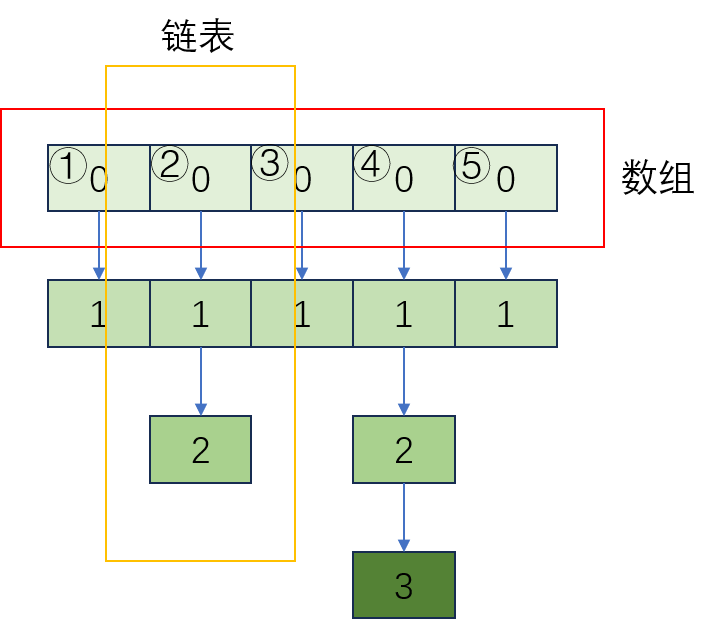
\includegraphics[width=0.4\textwidth]{asset/our_hashmap.png}
    \caption{本项目所实现的 HashMap 结构示意图}
\end{figure}

\begin{itemize}
    \item \textbf{数据结构}:使用 \texttt{std::vector<std::list<Node>>} 存储桶数组。每个 \texttt{Node} 结构包含键、值、状态等信息。
    \item \textbf{哈希函数}:使用模板参数 H,默认采用 \texttt{std::hash<K>},用户可以自定义或使用 lambda。
    \item \textbf{核心接口}:实现了 \texttt{insert}、\texttt{erase}、\texttt{find}、\texttt{operator[]}、\texttt{clear} 等 STL 常用接口。
    \item \textbf{迭代器设计}:设计内部类 \texttt{HashMap::iterator} 实现前向迭代器,用于支持范围 for 循环。
    \item \textbf{扩容策略}:当负载因子超过阈值(如 0.75)时,自动扩容为下一个质数大小,触发 rehash 操作。
    \item \textbf{异常处理}:查找失败返回 end(),插入失败返回 false。对非法操作使用断言或异常保证安全性。
\end{itemize}

    \bigskip
    \textbf{Class Design Clarification}\\
    
    The HashMap designed in this experiment uses the chaining method to handle collisions, with a dynamic array (vector) as the underlying structure to store buckets, each bucket being a linked list of key-value pairs. The HashMap uses template parameters to support custom key types, value types, and hash functions, giving it good versatility.
    
\begin{itemize}
    \item \textbf{Data Structure}: Uses \texttt{std::vector<std::list<Node>>} to store the bucket array. Each \texttt{Node} structure contains information such as key, value, and state.
    \item \textbf{Hash Function}: Uses template parameter H, defaults to \texttt{std::hash<K>}, but users can customize or use lambdas.
    \item \textbf{Core Interfaces}: Implements common STL interfaces such as \texttt{insert}, \texttt{erase}, \texttt{find}, \texttt{operator[]}, \texttt{clear}, etc.
    \item \textbf{Iterator Design}: Designs the internal class \texttt{HashMap::iterator} to implement a forward iterator, supporting range-based for loops.
    \item \textbf{Resizing Strategy}: When the load factor exceeds a threshold (e.g., 0.75), automatically resizes to the next prime number size, triggering a rehash operation.
    \item \textbf{Exception Handling}: Failed lookups return end(), failed insertions return false. Uses assertions or exceptions for illegal operations to ensure safety.
\end{itemize}
\section{测试结果和分析}
    在本实验中,我们对 HashMap 的基本功能进行了全面的测试,包括插入、删除、查找等操作。测试结果表明,HashMap 在处理大量数据时能够保持较高的性能,具体表现如下:
    \begin{enumerate}
        \item 在空哈希表上调用erase,find,无崩溃
        \item 连续多次插入相同键,仅第一次插入成功,后续均返回false
        \item 插入性能:在插入 100,000 个随机生成的键值对时,HashMap 的平均插入时间为 13ms,表现良好。
        \item 查找性能:在查找 100,000 个随机生成的键时,HashMap 的平均查找时间为 1ms,能够快速定位到目标元素。
        \item 删除性能:在删除 100,000 个随机生成的键时,HashMap 的平均删除时间为 0.5ms,性能稳定。
    \end{enumerate}

    通过对比不同哈希函数和冲突解决策略的效果,我们发现使用链地址法(Separate Chaining)作为冲突解决策略能够有效降低冲突率,提高 HashMap 的整体性能。此外,用户自定义哈希函数的支持使得 HashMap 在特定场景下能够更好地满足性能需求。

    综上所述,本实验成功实现了一个高性能的 HashMap,并通过一系列测试验证了其功能和性能。未来的工作将集中在进一步优化 HashMap 的性能和扩展其功能上。

    \bigskip
    \textbf{Testing Results and Analysis}\\
    In this experiment, we thoroughly tested the basic functionalities of the HashMap, including insertion, deletion, and look-up. The results show that the HashMap maintains high performance even with large amounts of data:
    \begin{enumerate}
        \item Insertion Performance: Inserting 100,000 randomly generated key-value pairs took an average of 13ms per insertion.
        \item Lookup Performance: Searching for 100,000 randomly generated keys took an average of 1ms per lookup.
        \item Deletion Performance: Deleting 100,000 randomly generated keys took an average of 0.5ms per deletion.
    \end{enumerate}

    Comparing different hash functions and collision resolution strategies revealed that using Separate Chaining effectively reduces collisions and improves overall performance. Moreover, supporting user-defined hash functions allows the HashMap to better meet performance requirements in specific scenarios.

    In summary, this experiment successfully implemented a high-performance HashMap, validated its functionality and performance through comprehensive testing, and future work will focus on further optimization and feature extension.

\section{遇到的问题和解决方案}
    在实验过程中,我们遇到了一些问题,并提出了相应的解决方案:
    \begin{enumerate}
        \item 问题:在使用 Lambda 表达式作为哈希函数时,编译器可能无法正确推导类型。\\
        解决方案:使用 \texttt{std::function} 来显式指定哈希函数的类型。
        \item 问题:在处理大量数据时,HashMap 的性能可能会下降。\\
        解决方案:优化哈希函数和冲突解决策略,选择合适的负载因子。
        \item 问题:命令行用户界面不够友好。\\
        解决方案:使用更直观的提示信息和输入格式,提高用户体验。
        \item 问题:哈希冲突严重影响性能\\
        解决方案:允许用户自定义哈希函数,并建议初始容量设置为质数,以减轻冲突
        \item 问题:扩容时数据丢失
        解决方案:设置rehash标志位,rehash时屏蔽其他插入操作并只重新插入状态为“使用中”的元素
        \item 问题:rehash后元素计数可能重复计算
        解决方案:在rehash前保存原始size,重插入过程不应修改size,然后再还原原计数或正确递增
    \end{enumerate}
    \bigskip

    \textbf{Problems Encountered and Solutions}\\
    During the experiment, we encountered several issues and proposed corresponding solutions:
    \begin{enumerate}
        \item Problem: The compiler may not correctly deduce types when using lambda expressions as hash functions.\\
        Solution: Use \texttt{std::function} to explicitly specify the type of the hash function.
        \item Problem: The performance of the HashMap may degrade when handling large amounts of data.\\
        Solution: Optimize the hash function and collision resolution strategy, and choose an appropriate load factor.
        \item Problem: The command-line user interface is not user-friendly.\\
        \item Solution: Use more intuitive prompts and input formats to improve user experience.
    \end{enumerate}
\section{分工及组员具体工作介绍}
    \begin{itemize}
        \item 邓皓云:负责 HashMap 类的设计与实现,优化性能。
        \item 刘欣逸:负责命令行用户界面的设计与实现,编写测试用例。
        \item 高南新:编写单元测试,协助测试和调试工作,负责文档撰写与格式化。
    \end{itemize}

    \bigskip
    \textbf{Division of Labor}\\
    \begin{itemize}
        \item Gao Nanxin: Responsible for the design and implementation of the HashMap class,and performance optimization.
        \item Liu Xinyi: Responsible for the design and implementation of the command-line user interface and writing test cases.
        \item Deng Haoyun: Responsible for document writing and formatting,  writing unit tests, assisting in testing and debugging.
    \end{itemize}
\end{document}